\documentclass[../main.tex]{subfiles}

\begin{document}

\section{Struktura zbiorów rozłącznych (DSU)}

\subsection{Wprowadzenie}

\begin{frame}{\subsecname}
  
Struktura zbiorów rozłącznych (ang. \textit{Disjoint Set Union} lub \textit{Union Find})
pozwalająca na 3 typy operacji:
\begin{itemize}
  \item \lstinline{make(v)}     -- tworzy nowy zbiór zawierający element $v$;
  \item \lstinline{union(v, u)} -- scala zbiory zawierające $v$ i $u$ w jeden;
  \item \lstinline{find(v)}     -- zwraca reprezentanta (zwanego też liderem) zbioru, do którego
                                   należy $v$.
\end{itemize}

\end{frame}

\begin{frame}{\subsecname}

Zbiory będziemy przechowywać w postaci drzew: każdemu drzewo będzie odpowiadało jednemu zbiorowi.
Korzeń drzewa będzie reprezentantem zbioru.

\begin{tikzpicture}

\begin{scope}[every node/.style={circle, draw,fill=gray!40}]
  \node[] (1) at (2,4) {1};
  \node[] (2) at (0,2) {2};
  \node[] (3) at (4,2) {3};
  \node[] (4) at (2,0) {4};
\end{scope}

\begin{scope}[every edge/.style={draw, thick, ->}]
  \only<2->\path (2) edge (1);
  \only<3->\path (4) edge (3);
  \only<4->\path (3) edge (1);
\end{scope}

\end{tikzpicture}

\end{frame}

\subsection{Naiwne rozwiązanie}

\begin{frame}[fragile]{\subsecname}

Bardzo łatwo można przechowywać ojca każdego wierzchołka (ojcem reprezentanta będzie on sam).

\pause
\begin{block}{}
\begin{lstlisting}[language = C++]
int rep[MAX_N];
int Find(int v) {
  return rep[v] == v ? v : Find(rep[v]);
}
void Union(int v, int u) {
  rep[Find(v)] = Find(u);
}
\end{lstlisting}
\end{block}

\pause
To rozwiązanie niestety może być czasem bardzo wolne. Nietrudno wymyślić przykład, w którym
drzewa będą formować długie łańcuchy. W pesymistycznym przypadku dla jednego zapytania mamy
złożoność $O(n)$.

\end{frame}

\subsection{Łączenie według rangi/rozmiaru}

\begin{frame}[fragile]{\subsecname}

W naiwnym rozwiązaniu zawsze dołączaliśmy lewy zbiór do prawego. Algorytm można znacząco
przyspieszyć, dołączając mniejszy ze zbiorów do większego lub tego z mniejszą rangą do tego z 
większą (ranga zbioru odpowiada wysokości drzewa).

\pause
\begin{block}{}
\begin{lstlisting}[language = C++]
struct { int rep, ranga; } f[MAX_N];
int Find(int v) {
  return f[v].rep == v ? v : Find(f[v].rep);
} |\pause|
void Union(int v, int u) {
  v = Find(v), u = Find(u);
  if (f[v].ranga > f[u].ranga) swap(v, u);
  f.rep[v] = u;
  f[u].ranga = max(f[v].ranga + 1, f[u].ranga);
}
\end{lstlisting}
\end{block}

\pause
Tak proste usprawnienie zbija złożoność do $O(\log{n})$.

\end{frame}

\begin{frame}{\subsecname}{Dowód złożoności}

Złożoność funkcji \lstinline{Union} jest w oczywisty sposób taka sama jak funkcji
\lstinline{Find}. Ta z kolei zależy jedynie od rangi zbioru. Naszym celem będzie udowodnienie, 
że w tak powstałych zbiorach $r(A) \le \log{|A|}$.\\
\pause
\begin{proof}[Dowód przez indukcje po rozmiarze zbioru:]{}
\begin{align*}
  |A| = 1 \implies r(A) = 0 \le \log{1} = \log{|A|}
\end{align*}
\pause
Bez straty ogólności niech $|A| \le |B|$, niech $T$ będzie zbiorem otrzymanym poprzez wykonanie
\lstinline{Union} na zbiorach $A$ i $B$.
\begin{align*}
  &r(T) = \max (r(B), 1 + r(A)) \le \max ( \log{|B|}, 1 + \log{|A|} )\\
  &\log{|B|} \le \log{(|A| + |B|)} \implies r(T) \le \log{(|A| + |B|)} = \log{|T|}\\
  &\log_2{2} + \log{|A|} = \log{(|A| \cdot 2)} \le \log{(|A| + |B|)} = \log{|T|}
\end{align*}
\end{proof}

\end{frame}

\subsection{Kompresja ścieżek}

\begin{frame}[fragile]{\subsecname}

Rozwiązanie można jeszcze bardziej usprawnić osiągając średnią złożoność rzędu $O(\alpha(n))$,
gdzie $\alpha(n)$ to odwrotna funkcja Ackermanna (dla $n\le 10^{600}, \alpha(n) \le 4$). Dowód
złożoności jest bardzo długi, więc go tutaj nie pokażę.\\
\pause
Usprawnienie wygląda tak:

\begin{block}{}
\begin{lstlisting}[language = C++]
int Find(int v) {
  return f[v].rep == v ? v
                       : f[v].rep = Find(f[v].rep);
}
\end{lstlisting}
\end{block}

\end{frame}

\end{document}
